\documentclass{article}
\usepackage{amsmath}
\usepackage{color}
\usepackage{graphicx}
\usepackage{epstopdf}
\usepackage{bm}
\begin{document}
\section{Problem}
Consider the following one-dimensional boundary point problem:
\begin{equation}\label{eq:2b}
\begin{cases}
&-\epsilon f''(x)+\epsilon \pi^2 f(x)+f'(x)=\sin \pi x\\
&f(0)=0,f(1)=0.
\end{cases}
\end{equation}
\section{asymptotic analysis}
Though the analytical solution can be solved explicitly, it is hard to analyze its behaviour without visualization.
By means of matched asymptotic expansion, we can find the ordinary solution away from $x=1$ satisfies:
\begin{equation}
\begin{cases}
&f'(x)=\sin \pi x\\
&f(0)=0
\end{cases}
\end{equation}
which can be solved trivally.
For the solution near x=1,let $\eta=\frac{1-x}{\epsilon}$, then
as $\epsilon \to \infty$, $f(\eta)$ satisfies 
\begin{equation}
\begin{cases}
&f_{\eta\eta}+f_{\eta}=-\epsilon(\pi^2 f+\sin \pi (1-\eta \epsilon))\\
&f_{|\eta=0}=0
\end{cases}
\end{equation}
The boundary condition at $\eta=0$ corresponds to $x=1$, to solve the leading order of the second equation, we need the second boundary condition,which can be obtained by matching the two solutions on the overlapping intervals.
As a result, first approximation of $f(x)$ is:
\begin{equation}
f(x)=\begin{cases}
\frac{1-\cos(\pi x)}{\pi}&0\leq x\leq 1-\epsilon\\
\frac{2}{\pi}(1-exp(\frac{x-1}{\epsilon}))&1-\epsilon\leq x\leq 1
\end{cases}
\end{equation}
\begin{figure}
\centering
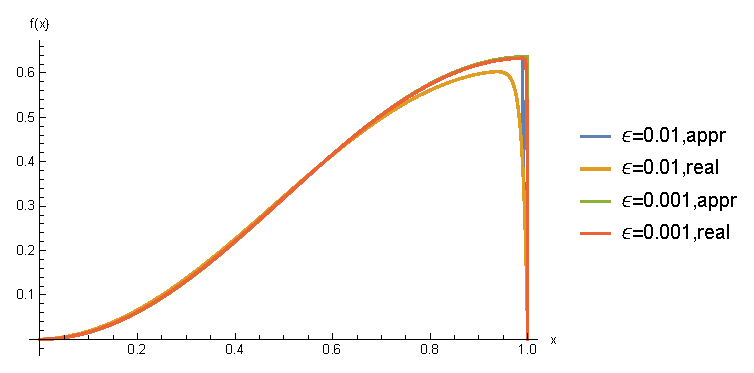
\includegraphics[width=\textwidth]{appr.eps}
\end{figure}
This piecewise expression for $f(x)$ is ambiguous near 1, since it is not continous at $x=1-\epsilon$. However, it illustrates two important facts:
\begin{itemize}
\item{the solution has boundary layer near $x=1$ and the thickness of the layer is $\epsilon$}
\item {the solution near 1 decrease \textcolor{blue}{exponentially} to 0(linearly as the first ordr of Taylor expansion).}
\end{itemize}
The asymptotic analysis before numerical solution gives important hints to narrow the mesh within boundary layer. Otherwise we cannot get good approximation to the real solution.
\section{numerical analysis}
We use finite element method to solve this problem.
First we split the interval $[0,1]$ into 
\[
0=x_0 < x_1 < \dots < x_{n-1} < x_n=1 
\]
and consider the space of piecewise linear functions determined by their values at $x_i$. The space has $n-1$ dimension such that we can find $n-1$ bases $\phi_i$, which satisfies:
\[
\pi_i(x_j)=\delta_{ij}
\]
We choose the best approximation for $f(x)$ from this $n-1$ dimensional space. To calculate the value of f(x) other than $x_i$, we use interpolating technique, which produces some errors. But even the solved $\hat{f}(x_i)$ is not accurate enough.

In this article, we leave the error analysis behind and give some numerical results concerning the finite element method.
First we transform the differential form (\ref{eq:2b}) to its 
weak formulation. 

Considering $\phi(x) \in \mathcal{C}^1$ and equals zero at 0 and 1. Then multiplying equation (\ref{eq:2b}) by $\phi(x)$ and integrating by parts, we get:
\begin{equation}
\epsilon\int_0^1 f'(x)\phi'(x)dx+\epsilon\pi^2\int_0^1 f(x)\phi(x)dx-\int_0^1\phi'(x)f(x)dx=\int_0^1\sin\pi x \phi(x)dx
\end{equation}
We chose $\phi(x)=\phi_i(x)$ respectively and write 
\begin{equation}
f(x)=\sum_i^{n-1}f(x_i)\phi_i(x)
\end{equation}
By elementary calculus we can get the equation system for $\bm{x}=(f(x_1),\dots,f(x_{n-1})^T$:
\begin{equation}
\bm{A}\bm{x}=\bm{b}
\end{equation}
where
$b_j=\int_0^1 \sin\pi x \phi_j(x)dx$
and
\begin{equation}
A_{ji}=\begin{cases}
\epsilon(\frac{1}{x_j-x_{j-1}}+\frac{1}{x_{j+1}-x_j})+\frac{\epsilon\pi^2}{3}(x_{j+1}-x_{j-1})&i=j
\\
-\frac{\epsilon}{x_{j+1}-x_j}+\frac{\epsilon\pi^2}{6}(x_{j+1}-x_j)+\frac{1}{2}&i=j+1
\\
-\frac{\epsilon}{x_j-x_{j-1}}+\frac{\epsilon\pi^2}{6}(x_{j}-x_{j-1})-\frac{1}{2}&i=j-1
\\
0&|i-j|>1
\end{cases}
\end{equation}
$\bm{A}$ is tri-dimensonal. The necessary condition for the stable solution is $A_{j,j+1}<0$, which gives $h \sim 2\epsilon$, where $h=\max |x_{i+1}-x_i|$. As a result, for a good approximation of real solution,the spatial step should be as small as $\epsilon$. 
\end{document}
